\documentclass[12pt]{report}
%\usepackage[francais]{babel}
\usepackage{lmodern}
\usepackage[a4paper]{geometry}
\usepackage[T1]{fontenc}
\usepackage[utf8]{inputenc}  
\usepackage{moreverb}
\usepackage{amsmath}
\usepackage{amsfonts}
\usepackage{amssymb}
\usepackage{textcomp}
\usepackage{pifont}
\usepackage{geometry}
\usepackage[pdftex]{graphicx}
\usepackage{graphics}
\usepackage{url}
\usepackage{graphicx}
\usepackage{float}
\usepackage{color}
\usepackage[nottoc, notlof, notlot]{tocbibind}
\usepackage[french]{varioref}
\usepackage[Glenn]{fncychap}
\usepackage{pdfpages}

\usepackage{multicol}

% entête et pied de page
%% \usepackage{fancyhdr} 
%% \pagestyle{fancy}
%% \renewcommand{\chaptermark}[1]{\markboth{#1}{}}
%% \renewcommand{\sectionmark}[1]{\markright{\thesection\ #1}}
%% \fancyhf{} \fancyhead[LE,RO]{\bfseries\thepage}
%% \fancyhead[LO]{\bfseries\rightmark}
%% \fancyhead[RE]{\bfseries\leftmark}
%% \renewcommand{\headrulewidth}{0.5pt}
%% \addtolength{\headheight}{0.5pt}
%% \renewcommand{\footrulewidth}{0pt}
%% \fancypagestyle{plain}{ \fancyhead{}
%% \renewcommand{\headrulewidth}{0pt}} 

% pour inclure du code par exemple
\usepackage{listings}

\lstset{%configuration de listings
float=hbp,%
basicstyle=\ttfamily\small, %
columns=flexible, %
tabsize=2, %
frame=trBL, %
frameround=tttt, %
extendedchars=true, %
showspaces=false, %
showstringspaces=false, %
numbers=left, %
numberstyle=\tiny, %
breaklines=true, %
breakautoindent=true, %
captionpos=b,%
xrightmargin=0cm, %
xleftmargin=-0cm, %
language=tex, %
frameround=fttt;%
}

%%%%%%%%%%%%%%%% Lengths %%%%%%%%%%%%%%%%
\geometry{a4paper,twoside,left=2cm,right=2cm,marginparwidth=1.2cm,marginparsep=3mm,top=1.7cm,bottom=1.5cm}

\newcommand{\stamp}{{\tt \textit{Stamp }}}
\newcommand{\class}{{\tt \textit{class }}}
\newcommand{\initarg}{{\tt \textit{Initarg }}}
\bibliographystyle{plain}
\urlstyle{sf}

%%%%%%%%%%%%%%%%%%%%%%%%%%%%%%%%%%%%%%%%%%%%%%%

\newenvironment{vcenterpage}
{\newpage\vspace*{\fill}}
{\vspace*{\fill}\par\pagebreak}

\newtheorem{ex}{Exemple}%[section]
\newtheorem{theo}{Theorem}
\newcommand{\tuple}[1]{\ensuremath{\langle #1 \rangle}}

\begin{document}
%%%% Page de titre %%%%
\def\logo{
  \begin {figure}[H]
	
\includegraphics[scale=0.33]{\DIR/img/logo.jpg}
        \hspace{1cm}
        
\includegraphics[scale=0.2]{\DIR/img/logobordeaux1.jpg}
        \hspace{2.8cm}
        
\includegraphics[scale=1]{\DIR/img/logoEvollis.png}        
        \hspace{0.8cm}   
        
\includegraphics[scale=0.3]{\DIR/img/logoLaBRI.jpeg}	

	\label{logo}
  \end {figure}
}

\def\title{Mise en place d'une solution non relationnelle de gestion de données}

\def\intervenant{
        \begin{flushleft}
	  \begin{tabbing}
		\textbf{Maître de stage:}
                \hspace{7.2cm} \=\textbf{Étudiant:} \\
                \noindent Eric de {\sc Marignan}
                \> {\sc Barro} Lissy Maxime\\
                \> \\
                \noindent \textbf{Tuteur à} {\sc bordeaux}1 {\bf :}
                \> Élève ingénieur\\
                \noindent Mohamed {\sc Mosbah}
                \> Dernière année - Option GL \\ 
                \noindent Sofian {\sc Maabout} \> {\sc enseirb-matmeca} 2011/2012 \\
                \>\\
                \noindent \textbf{Tuteur à l'{\sc enseirb}:}
                \> \\
                %\noindent aaaa {\sc aaaa}
	  \end{tabbing}
        \end{flushleft}
}

\def\date{\today}%9 juin 201}

\def\job{PROJET DE FIN D'ÉTUDE / STAGE MASTER 2 RECHERCHE}

\begin{titlepage}
  \logo
  \begin{flushleft}
    \textbf{École Nationale Supérieure d’Électronique, Informatique,
      Télécommunications, Mathématique et Mécanique de Bordeaux}

    \vspace{0.5cm}

    \textsf{Département informatique}

    \vspace{0.5cm}

   1 avenue du Dr Albert Schweitzer\\
   B.P. 99 33402 Talence Cedex

    
  \end{flushleft}
  
  \vspace{4cm}
	\begin{center}
	  {\bf \job}\\
	  \vspace{1cm}
		 {\LARGE\bf \title}\\
\vspace{1cm}
           \date

	\end{center}


        \vspace{4cm}
        \intervenant
\end{titlepage}


%%%% remerciement %%%%%%%
% \chapter*{Thanks}

% \addcontentsline{toc}{chapter}{Thanks}

%%%%% terminologie %%%%%%%%%%
%% \newpage

\def\termea{\bf \footnotesize xx}
\def\sensa{\footnotesize xx}

\def\termeb{\bf \footnotesize xx}
\def\sensb{\footnotesize xx}

\def\termec{\bf \footnotesize xx}
\def\sensc{\footnotesize xx}

\def\termed{\bf \footnotesize }
\def\sensd{\footnotesize }

\def\termee{\bf \footnotesize }
\def\sense{\footnotesize }

\def\termef{\bf \footnotesize }
\def\sensf{\footnotesize }

\def\termeg{\bf \footnotesize }
\def\sensg{\footnotesize }

\def\termeh{\bf \footnotesize }
\def\sensh{\footnotesize }

\def\termei{\bf \footnotesize }
\def\sensi{\footnotesize }

\def\termej{\bf \footnotesize }
\def\sensj{\footnotesize }

\def\termek{\bf \footnotesize }
\def\sensk{\footnotesize }



\begin{center}
\subsubsection*{Terminologie}
\begin{tabular}{|p{5cm}|p{12cm}|}
\hline
{\bf ~~~~~ T{\scriptsize ERME}} &  {\bf ~~~~~~~~~~~~~~~~~~~ S{\scriptsize IGNIFICATION}}\\
\hline
\hline
\termea & \sensa\\
\hline
\termeb & \sensb\\
\hline
\termec & \sensc\\
\hline
\termed & \sensd\\
\hline
\termee & \sense\\
\hline
\termef & \sensf\\
\hline
\termeg & \sensg\\
\hline
\termeh & \sensh\\
\hline
\termei & \sensi\\
\hline
\termej & \sensj\\
\hline
\termek & \sensk\\
\hline

\end{tabular}
 
\end{center}


%%%% resume %%%%%%%%%
\begin{abstract}
  The article we worked on deals with how to visualize graphs containing many nodes and edges. With huge amounts of data generally comes visual clutter, in our case due to edge crossing. This solution is based on an edge bundling technique coupled with a grid built from the original graph. Our solution uses the Tutte algorithm in order to quickly obtain a graph without crossing, based on a triangular-face grid, which helps to read relationships between nodes. Moreover, this method will uniformize edge length to ease the visualization. This algorithm is available as a standalone program for Tulip. 

\end{abstract}

%%%% plan %%%%%
\tableofcontents
%\listoffigures
%\listoftables



%%%%% corps du rapport %%%%%%%%%
\chapter*{Introduction}

The article ~\cite{pd} talks about how to visualize graphs containing many nodes and edges. Improvements in data acquisition leads to an increase of the size and the complexity of graphs and this huge amount of data generally causes visual clutter, in our case due to edge crossing.
For example, it could be interesting to visualize data in fields like biology, social sciences, data mining or computer science, and then emphasize their high-level pattern to help users perceive underlying models.


Nowadays, in the research world, the information is easily represented into graphs to visualize more and more data. However, this huge amount of information prevents the graph from being manually drawn:  It explains the need of automatic methods able to generate an appropriate graph with all nodes and edges. Yet this graph may suffer from cluttering, which should be reduced for a better understanding.

Our objective all along this project is to read what has been done before relating to this problem, to provide an objective point of view on those previous works, and propose our contribution. We have implemented a method, then optimized its performances with
 current technologies (OpenMP, Tulip...) and setted our boundaries. 


The first part of this document presents review-related work on reducing edge clutters and enhancing edge bundle visualization, with which the article is connected. The second will deal with the Tutte algorithm and its differents versions. A third part will talk about the implementation issues and show our results. Finally, we draw a conclusion and explain the limits of our work for further improvements.

\addcontentsline{toc}{chapter}{Introduction}


\chapter{The context}

\textbf{Some classes of graph}, such as trees or acyclic graphs, clearly facilitate user understanding by effective representation. However, most graphs do not belong to these classes, and algorithms giving nice results in terms of time and space complexity but also in terms of aesthetic criteria for any graph do not exist yet. For example, the force-directed method produces pleasant and structurally significant results but does not help user comprehension due to data complexity. The authors of the paper specify two techniques for that reduction: compound visualization and edge bundling. But their interest goes to Edge Bundling, which suggests to route edges into bundles in order to uncover high-level edge patterns and emphasize information.~\cite{pd, pe} Their contribution was to set this edge bundling by discretizing the plane into a new mesh.
%domain where the graph is set so that boundaries of the new discretization are formed.
\\
\\
\textbf{Up to now}, several techniques have been used to reduce this clutter, based on compound visualization or edge bundling. In a compound visualization, nodes are gathered into metanodes and inter-cluster edges are merged into metaedges. To retrieve the information, metanodes could be collapsed or expanded. Yet an important constraint is the impossibility for some nodes to move while avoiding edges crossing because node positions provide information: consequently, compound visualization is not suitable. To reduce visual clutter, another clue is to keep vertices while edges are aggregated: the Edge bundling technique routes edges into bundles. This uncovers high level edge patterns and emphasizes relationships. Moreover, some existing representations take into account the the inability of some nodes to change position i.e.  some reducing edge clutters (Edge routing, Interactive techniques, Confluent Drawing, Edge clustering) and other enhancing edge bundles visualizations (Smoothing curves, Coloring edges). 
\\
\\
\textbf{The publication we are currently working on} is based on a new edge bundling algorithm for efficient graph drawing. By using specific  discretization methods such as quad-tree and Voronoï diagrams which are little time-consuming calculations, the authors obtained a new separation of the region where they can reduce the drawing area. As a result, their final discretization algorithm is a good trade off between good precision($quad~tree$) and the computation time ($Voronoï$)[$ref$].

% and Bezier curves to visualize aesthetic graphs.

In order to create the Edge-bundling effects, the authors use the "shortest path" Dijskstra  algorithm. But this does not create a decent number of bundles. Then they add new concepts such as $roads$ and $Highways$ to increase this number. This means to reduce the weight of an edge (of the grid obtained before) if it is highly used, but only after computing several shortest paths between linked nodes of the original graph. 

  Several optimizations of the specific shorstest path algorithm such as function calls reductions, multithreading reduces tremendously computation time of graphs.


The authors of the article, after the rendering of their algorithm, think that their grid can be improved because what they have got presents some inconveniences such as the big amount of bends ("zigzag" effect on the grid) and irregular triangles. To solve those problems, they want a heuristic to uniformize sizes of the edges and increase angles between edges that harm graph reading. The proposition in our work is the use of  the Tutte algorithm which is only applicable for an internally triangulated planar graph and renders more informative and aesthetic graphs (Less edge crossing, less bends, smaller sizes of edges, maximum angular resolution).


%\chapter{Previous works}

\chapter{Tutte}

\section{Tutte's algorithm}

The basic graph theory terminology defined in the article ~\cite{pa, pb}
will be used.  Let $G=(V,E)$ be a planar graph. A mapping $\Gamma$ of $G$
into the plane is a function $\Gamma : V \cup E \to P(\mathbb{R}^2)$. This
function maps a vertex $v \in V$ to a point in $\mathbb{R}^2$ and an edge
$e = uv \in E$ to the straight line segment joining $\Gamma(u)$ and
$\Gamma(v)$.  A mapping is an embedding if distinct vertices are mapped to
distinct points and the open segment of each edge does not intersect any
other open segment of an edge or a vertex.
\\

A way to build embeddings of any planar, 3-connected graph $G=~(V,E)$ have
been produced by Tutte in 1963 ~\cite{pc}. Let $C$ be a cycle of
vertices. Those vertices are the vertices of a face of G in some (not
necessarily straight-line) embedding of $G$. Let $\Gamma$ be a mapping of
$G$ into the plane.

% In 1963, Tutte~\cite{pc} gave a way to build embeddings of any planar,
% 3-connected graph $G=~(V,E)$. Let $C$ be a cycle whose vertices are the
% vertices of a face of G in some (not necessarily straight-line) embedding
% of $G$. Let $\Gamma$ be a mapping of $G$ into the plane, satisfying the
% conditions:

% \begin{itemize}

% \item the set Ve of the vertices of the cycle C is mapped to the vertices of a strictly
% convex polygon Q, in such a way that the order of the points is respected;

% \item each vertex in $V_i = V \ V_e$ is a barycenter with positive coefficients of
% its adjacent vertices (Tutte assumed all coefficients to be equal to 1, but
% the proof extends without changes to this case). In other words, the images
% v of the vertices v under $\Gamma$ are obtained by solving a linear system
% (S): for each $u \in V_{i, v|uv \in E} \lambda_{uv} (u - v) = 0$, where the
% $\lambda_{uv}$ are positive reals. It can be shown that the system (S) admits
% a unique solution.

% \end{itemize}

\begin{theo} \label{theo:box} (Tutte’s Theorem) Let $Ve$ be a set of the
  vertices of the cycle $C$ mapped to the vertices of a strictly convex
  polygon $Q$, in such a way hat the order of the points is respected.  If
  for each vertex in $V_i = V \ V_e$ is a barycenter with positive
  coefficients of its adjacent vertices (Tutte assumed all coefficients to
  be equal to 1, but the proof extends without changes to this case), so
  $\Gamma$ is an embedding of $G$ into the plane, with strictly convex
  interior faces.
\end{theo}

\begin {figure}[H]
  \centering
  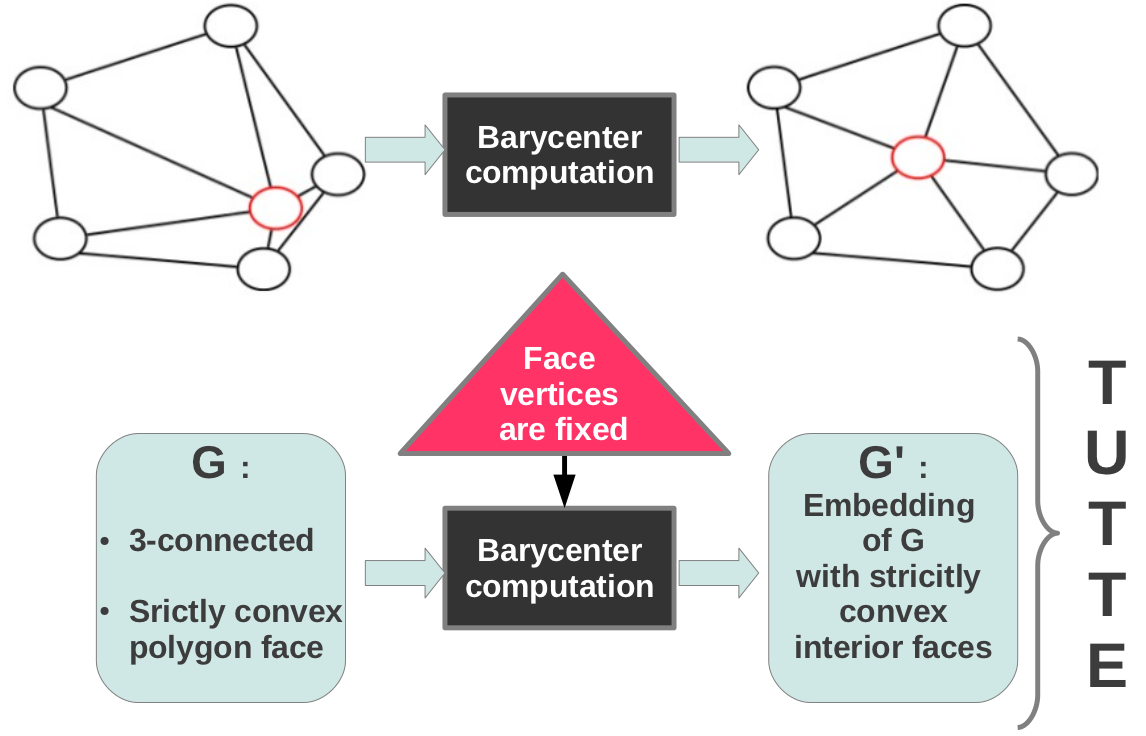
\includegraphics[scale=0.3]{img/tutte.png}
  \caption{Tutte's theorem illustration}
  \label{struct3}
\end {figure}

\subsection{Some extreme cases about Tutte's theorem}
In our project we do not use 3-connected graph but graph whose interior faces are triangle. It is obvious that considering the kind of graphs we used Tutte's theorem is verified because the hypothesis « All interior faces are tringle » is lighter than « 3-connected » hypothesis. So now we changed the hypothesis about the external polygon and the interior vertices in order to find out if the tutte's  is always verified.  

\subsubsection{Tutte's theorem and concave polygon}

In this section, we changed the hypothesis about the graph face. Now we consider a concave polygon face. Below is the illustration of a couterexample. 

\begin {figure}[H]
  \centering
  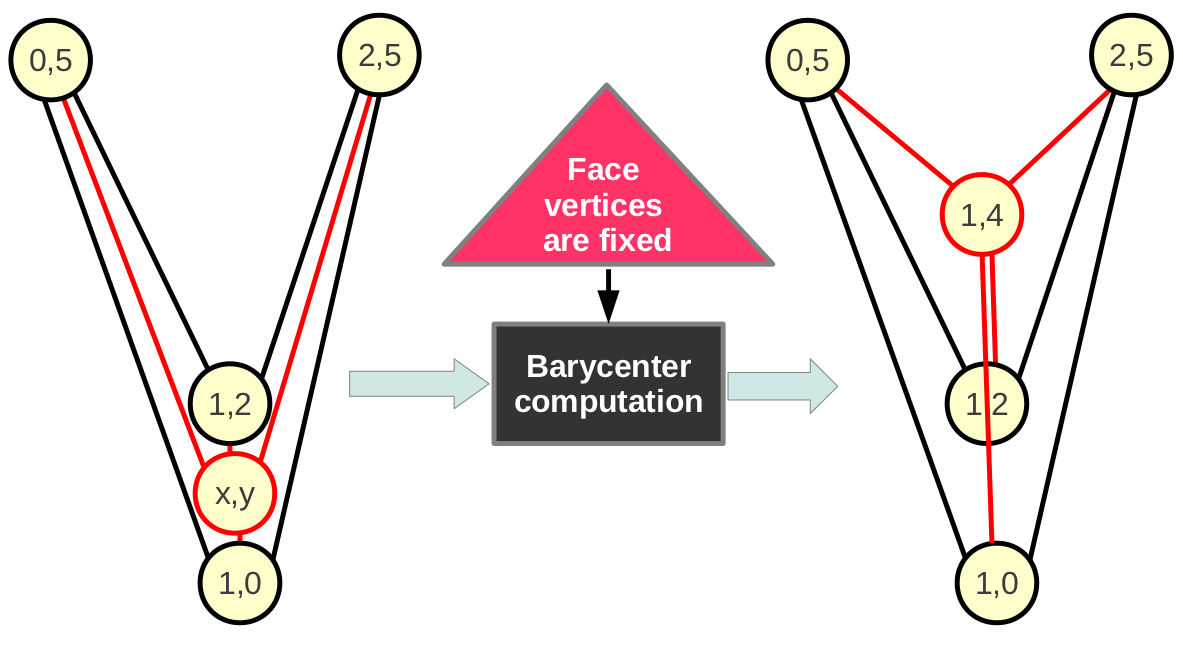
\includegraphics[scale=0.3]{img/tutte2.png}
  \caption{Tutte algorithm on concave polygon}
  \label{tutte2}
\end {figure}
\noindent
In the counterexample illustration above, the coordinate of the vertex shown in red color become $$(\frac{0+1+1+2}{4} , \frac{5+0+2+5}{4}) = (1 , 4)$$
One can see that after the barycenter algorithm computation, the graph is no longer embedding. So the Tutte's theorem is not verified considering graphs with concave polygon face. 

\subsubsection{Tutte's algorithm and convex polygon with some fixed vertices}
This section kept the «convex polygon face» hypothesis but some internal vertices are considered fixed, their position never change during the barycenter algorithm computation. Below is the illustration of a couterexample. 

\begin {figure}[H]
  \centering
  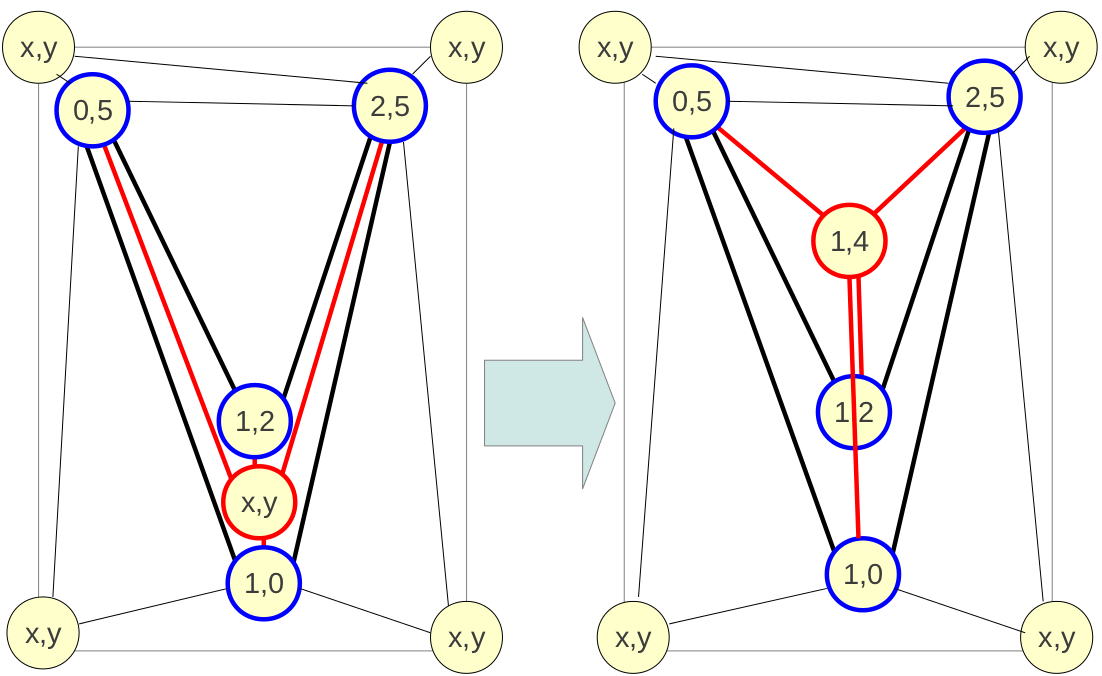
\includegraphics[scale=0.3]{img/tutte3.png}
  \caption{Tutte algorithm on convex polygon and fixes vertices}
  \label{tutte3}
\end {figure}
\noindent

As in the previous counterexample illustration (fig \ref{tutte2}) above, after the barycenter algorithm computation, the vertex shown in red color position changes. So the graph is no longer embedding which implies that the Tutte's theorem is not verified considering that some internal vertices can be fixed.


% \begin{thebibliography}{99}

% \bibitem{pa} E. Colin de Verdière, M. Pocchiola, and G. Vegter. Tutte's Barycenter Method applied to Isotopies. \emph{Computational Geometry: Theory and Applications, 26}, 81–97, 2003.

% \bibitem{pb} B. Bollob's. Modern graph theory, \emph{volume 184 of Graduate Texts in Mathematics}. Springer-Verlag, 1998.

% \bibitem{pc} W. T. Tutte. How to draw a graph. \emph{Proceedings of the London Mathematical Society}, 13:743–768, 1963.

% \end{thebibliography}




\section{Tutte's Sequential Algorithm}

To obtain the graph resulting from the Tutte theorem, an algorithm is
needed. In this section, a sequential algorithm is described. This
algorithm is an iterative solution. To compute a solution, a set of nodes
 making up a convex polygon must be decided. Let $P$ be this set of nodes. Let
$G_k$ be the graph generated at the step $k$.
\\

To obtain the graph of the next step, all the nodes of the interior of the
convex polygon $P$ will be visited. For each node visited, the barycentric
coordinates of its neighbourhood are computed. Then these coordinates are used
to update the position of the current node. Once each node has been visited,
the computation of the graph $G_{k+1}$ is completed.
\\
In this project, the stop condition used for this algorithm is an epsilon
between the relative positions of the node of the graph $G_k$ and
$G_{k+1}$. For all nodes of the graph, if the length of each movement is
inferior to a given epsilon, the graph $G_{k+1}$ is the solution.
\\

The figure \ref{transition} gives an exemple of the mouvement of one node
during one step.
\begin{figure}[!h]
\centering
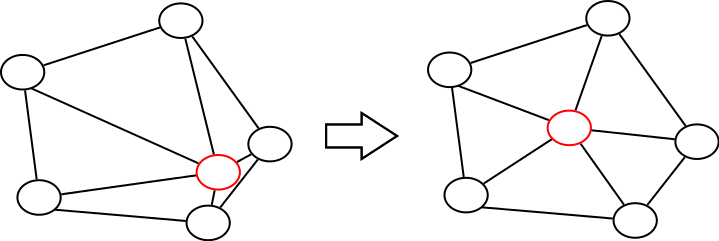
\includegraphics[scale=0.5]{img/transition.png}
\caption{barycenter computation of the red node}
\label{transition}
\end{figure}

This gives a synthetic view of this algorithm : 
\begin{verbatim}
G = {V,E}
P = set of nodes constituent a convex polygon
procedure tutte(G, P, epsilon)
  epsilon_current = 0
  for each node of (V \ convex polygon)
    barycenter = barycenter of neighboring nodes
    epsilon_current = max(epsilon_current, distance(node, barycenter))
    node = barycenter
  if (epsilon_current < epsilon)
    exit()
  tutte(G, P, epsilon)
\end{verbatim}

From the complexity point of view, during one iteration all the nodes of
the set $V$ - $convex~polygon$ are visited. For each node, all its
neighbourhood is visited. Let $mean\_d$ be the average degree of this planar
graph. So the compexity of an iteration is $\mathit{O(n \times mean\_d)}$
with $n = |V|$.

% Le but ici est d'exposé la méthode algorithmique qui découle de l'algorithme de Tutte et  de prouver que cette méthode converge (retrouver l'article qui en parle)


\section{Tutte Parallel Algorithms}
%here should be the implementation of Tutte with basic structure 


%\subsection{Sequentiel version}
%in this first optimization Frozar you are suggested to put the improvement due to the new data structure you took
In the sequential version, the algorithm presented is an asynchronous Tutte one. In fact, there is a second approach, the synchronous Tutte version. The difference between the two approaches is :
\begin{itemize}
\item in asynchronous version: each movement is applied directy after being computed
\item in synchronous version: all movement are computed before being applied
\end{itemize}
In the sequential version, the synchronous approach does not present
benefits. It is more convenient to consider neighbors movement.

In the parallel version, the synchronous approach may be interesting in
order to reduce critical sections. For the both parallel approach use the
OpenMP library.
\\
The complexity these two algorithms is roughly $\mathit{O(\frac{n}{p})}$
with $n = |V|$ and $p$ is the number of processeurs.
\\

\subsection{Asynchronous parallel version}
% in this optimization Ozenati you are suggested to talk about the
% asynchronous implementation (if faster than the others) with graph
% coloration
\subsubsection{Distribution of nodes: Graph coloring}
In order to implement a parallel asynchronous version of the Tutte algorithm, it is necessary to separate graph nodes into different sets. The objective is to extract an independence between nodes. In fact, each node has to move while the neighbours maintain their positions. Thus, the independence must be between the moving node and its neighbours. This problem is similar to the famous problem of graph coloring.
\paragraph*{}
The objective of the modified Tutte algorithm is to handle graphs of thousands of nodes. To separate such a number of nodes, it is more effective to use a heuristic of the algorithm of graph coloring.\\
The greedy algorithm is a simple and good solution to separate nodes into sets fast and effectively.~\cite{pf}
\paragraph*{}
The algorithm used in this project is :
\begin{verbatim}
G={V,E}
Y = V
color = 0
While Y is not empty
   Z = Y
   While Z is not empty
      Choose a node v from Z
      Colorate v with color
      Y = Y - v
      Z = Z - v - {neighbors of v}
   End while
   color ++
End while
\end{verbatim}

This algorithm is known to use at most $d(G)+1$ colors where $d(G)$ represents the largest value of the degree in the graph G. However, its shortcoming is that it produces sets of different size. This can be inconvenient for task distribution.
\subsubsection{Applying Tutte algorithm to sets}
Once a set of nodes is obtained, it is possible to apply a parallel Tutte algorithm. The question is how to parallelize it on sets of nodes. The natural idea is to attribute one set per thread :
\begin{figure}[!h]
\centering
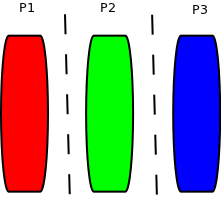
\includegraphics[scale=0.5]{img/distribution_verticale.png}
\caption{One set per thread}
\end{figure}
This distribution is far from being optimal. In fact, each thread has to lock the neighbours nodes before moving the concerned node, which introduces an important critical section. In addition to being unfair, this distribution is limited by the number of sets produced.\\

The best distribution for sets obtained by graph coloring is to execute $n$ threads on one set. Each thread moves a number of nodes of the set without any critical section, since each node of the set is not the neighbour of all the other nodes of the same set. Once the thread has moved all its nodes of the set, it must wait for other threads to have completed the same process (implemented by a barrier). Then, the overall process is applied to the next set.

\begin{figure}[!h]
\centering
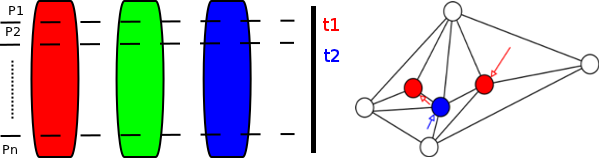
\includegraphics[scale=0.5]{img/distrib.png}
\caption{$n$ threads per set}
\end{figure}





\subsection{Synchronous parallel version}

The parallel synchronous version of the Tutte algorithm is easier to
implement then the parallel asynchronous. For this version, one
does not need to compute a coloring separation.
\\

During an iteration, the new coordinates of all nodes on the graph are saved in a table instead of being
directly applied. At the end of an iteration, all upgrades are applied. In
this approach, two nodes can be computed independently in parallel. 
\\

Consequently, for an iteration, the set of nodes to visit can be separated in different
subsets. Each of these subsets is independent and can be computed by
different threads in parallel. The separation is static, i.e. the number of
element of each subset is equal to $nb\_node / nb\_thread$.



\chapter{Implementations}

%\section{Graph representation for Tulip}

%it is asked here to talk about the situation of the graph is before we start the implementation: how do we manage to have the graph

%It is asked here to talk briefly about the algorithm we are going to use in the project: how it works (hope you see what I mean) 


\section{Data Structure}
%here sould be presented the first data structure used
In the implementation of our solution we have defined our own data
structure on which we execute the Tutte algorithm. We have
implemented some mechanisms to convert a tulip format graph to our own
graph structure and also to get information from our structure to insert them 
into a Tulip graph. In other words, our structure is a
temporary structure for storing information about nodes in order to
execute the Tutte algorithm.

\subsection{Issues}
As the Tulip data structure contains a lot of information, it is
expensive to manipulate them. Furthermore, we do not need all the
information from a given Tulip graph. For
instance, for a given node, we just want to know if it is fixed. For a
fixed node, position never changes during the Tutte algorithm. In
addition to that, as we are looking for performance, we need a light
structure matching the principe of Tutte algorithm. The following
points are the main reasons which lead us to set up a new data
structure.
\begin{enumerate}
\item The fact that a given node is fixed or not is indicated firstly
  by a mobility property. However, there is another property indicating
  nodes which are part of graph contouring, and these nodes need to be
  fixed too. Therefore, to deal with the fact that a given node is fixed or
  not, we need to manipulate two properties that cost a lot.

\item In Tulip data structure there is a hierarchy of graphs. However, we only need
  the parent of the graph. We do not need the sub-graph relation between graphs.

%%, the one which is not subgraph of another
  %%one
%% \item The informations about nodes are not in node but there is a
%% map between nodes and properties. For a given node, it cost a lot
%% to acces to one of its properties.

\end{enumerate}  

\subsection{Implementations}
We tested three implementations in order to find out the right one. Because we care of memory and speed, we merely store only the information needed to run the algorithm in our structure.

\subsubsection{First implementation}
In this implementation, our structure is constructed so that a given node
contains its neighbourhood. So one can easily access the neighbourhood
of a given node because it is very crucial in a Tutte algorithm
implementation. To do this, we define a class that contains the various
data needed on a given node (the attributes) and all the operations we
need to run on a node (the methods).

\newpage
\begin{lstlisting}
class MyNode {
 private:
  node n;
  bool mobile;
  Coord coord;  
  vector<MyNode *> voisin;

 public:
  MyNode();
  MyNode(const node n, const Coord coord);
  MyNode(const node n, const bool mob, const Coord coord);
  ~MyNode();
  
  const node getNode() const;
  bool getMobile() const;
  void setMobile(const bool b);
  const Coord getCoord() const;
  void setCoord(const Coord &);
  vector<MyNode *> * getVoisin();
  vector<MyNode *> getVoisin() const;
};
\end{lstlisting}
\noindent
\underline{\bf Vertex attributes needed}
\begin{dinglist}{70}
\item[n]: \texttt{node} type of \textsf{Tulip} library; contains the \texttt{ID} of the node.  
\item[mobile]: \texttt{boolean} type; is used to know a given node is considered fixed.
\item[coord]: \texttt{Coord} type of \textsf{Tulip} library; is used to store the node coordinates. 
\item[voisin]: \texttt{vector} type of \texttt{C++} library; contains the neighbourhood.
\end{dinglist}
\noindent
\underline{\bf Operations on a vertex}~\\
We used two types of operations or methods: \textsf{setter} and
\textsf{getter}. A \textsf{setter} is a method used to set the value of an
attribut and a \textsf{getter} is used to get the value of an attribut. For
a given attribut \texttt{attribut} , the corresponding setter and getter
are respectively \verb+setAttribut(args)+ and \verb+getAttribut()+. Below
are the lists of the setters and getters of nodes in our structure:
\begin{dinglist}{70}
\item[Setters]: \verb+getMobile(), getCoord(), getVoisin()+  
\item[Getters]: \verb+setMobile(const bool b), setCoord(const Coord &), getVoisin()+.
\end{dinglist}

\subsubsection{Second implementation}
In the second implementation, the built data structure aims to decrease
the number of pointer translation of the system. Also, the method to fill
our data structure tries to put the neighbourghood coordinates of a node 
near to its own.

A new basic class of MyNode\_ver2 have been implemented. The vector \\
\verb+vector<MyNode *> voisin+ is substituted by an integer \verb+index_neighbourhood+.

Here is the statement of this class:

\newpage
\begin{lstlisting}
  class MyNode_ver2 {
    public:
    node n;
    bool mobile;
    int index_neighbourhood;
    int degree;
  };
\end{lstlisting}

To store all the nodes, the neighboughoods and the coordinates, three tables are needed. 

\begin{lstlisting}
  vector<MyNode_ver2> MyNodes_2;
  vector<int> Neighbourhoods;
  vector<Vec2f> * coords;
\end{lstlisting}

\begin{dinglist}{70}
\item[MyNodes\_2]: contains all the nodes.
\item[Neighbourhoods]: contains the index of all the neighbourhoods.
\item[coords]: is used to store the nodes coordinates. 
\end{dinglist}

The attribute \verb+index_neighbourhood+ of the class \verb+MyNode_ver2+
gives the index of the neighbourhood of the node in the vector \verb+Neighbourhoods+.

\subsubsection{Third implementation}
In this third implementation, we do not use a class to store the
various data about node to run Tutte algorithm. 
As we are looking for a lighter data structure in order to ameliorate 
memory access, we use a \textsf{struct} to group data needed about a given node
under one name (\textsf{Data}). 
\begin{lstlisting}
  struct Data {
    node n;
    Coord coord;
    bool mobile;
  } Data;
\end{lstlisting}
In addition of the structure above, we use two tables: a \texttt{data store table} table to store data about nodes and \texttt{neighbourhoods table} to link nodes with their neighbourhoods. The picture below illustrate the principle.
\begin {figure}[H]
  \centering
  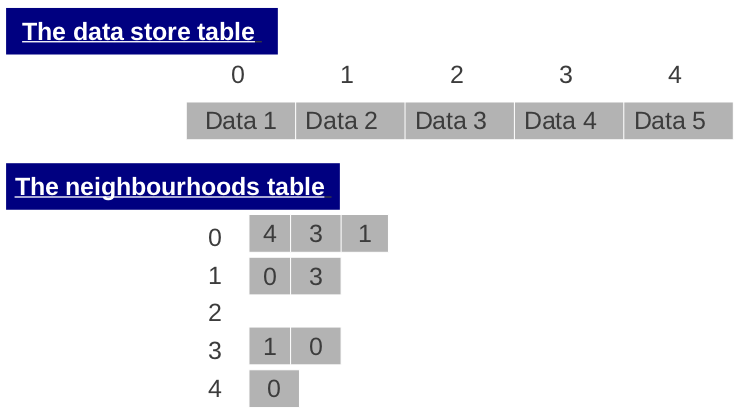
\includegraphics[scale=0.5]{img/struct3.png}
  \caption{Third implementation graph representation}
  \label{struct3}
\end {figure}
\noindent One can read in the \texttt{neighbourhoods table} that neighbours of the node 0 are nodes \texttt{4, 3,  1} and node 2 does not have neighbours. One can access all information about node 0 located at the index 0 of the \texttt{data store table}.  
%\subsection{Enhanced implementation}

%% \subsubsection{Distribution of nodes: Graph coloring}
In order to implement a parallel asynchronous version of the Tutte algorithm, it is necessary to separate graph nodes into different sets. The objective is to extract an independence between nodes. In fact, each node has to move while the neighbours maintain their positions. Thus, the independence must be between the moving node and its neighbours. This problem is similar to the famous problem of graph coloring.
\paragraph*{}
The objective of the modified Tutte algorithm is to handle graphs of thousands of nodes. To separate such a number of nodes, it is more effective to use a heuristic of the algorithm of graph coloring.\\
The greedy algorithm is a simple and good solution to separate nodes into sets fast and effectively.~\cite{pf}
\paragraph*{}
The algorithm used in this project is :
\begin{verbatim}
G={V,E}
Y = V
color = 0
While Y is not empty
   Z = Y
   While Z is not empty
      Choose a node v from Z
      Colorate v with color
      Y = Y - v
      Z = Z - v - {neighbors of v}
   End while
   color ++
End while
\end{verbatim}

This algorithm is known to use at most $d(G)+1$ colors where $d(G)$ represents the largest value of the degree in the graph G. However, its shortcoming is that it produces sets of different size. This can be inconvenient for task distribution.
\subsubsection{Applying Tutte algorithm to sets}
Once a set of nodes is obtained, it is possible to apply a parallel Tutte algorithm. The question is how to parallelize it on sets of nodes. The natural idea is to attribute one set per thread :
\begin{figure}[!h]
\centering
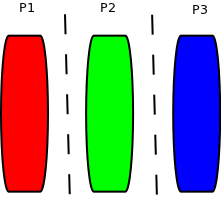
\includegraphics[scale=0.5]{img/distribution_verticale.png}
\caption{One set per thread}
\end{figure}
This distribution is far from being optimal. In fact, each thread has to lock the neighbours nodes before moving the concerned node, which introduces an important critical section. In addition to being unfair, this distribution is limited by the number of sets produced.\\

The best distribution for sets obtained by graph coloring is to execute $n$ threads on one set. Each thread moves a number of nodes of the set without any critical section, since each node of the set is not the neighbour of all the other nodes of the same set. Once the thread has moved all its nodes of the set, it must wait for other threads to have completed the same process (implemented by a barrier). Then, the overall process is applied to the next set.

\begin{figure}[!h]
\centering
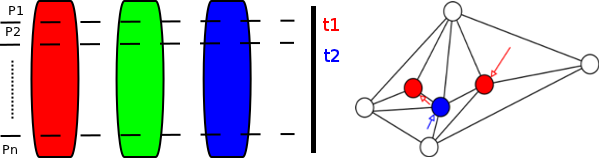
\includegraphics[scale=0.5]{img/distrib.png}
\caption{$n$ threads per set}
\end{figure}





\section{Results}
\subsection{Benchmark}

The authors provided us with three graphs in order to test our
different implementations of the Tutte method.\\

These graphs have the following characteristics :

\begin{center}
\begin{tabular}{|c|c|c|}
\hline
Graph & number of vertices & number of edges \\
\hline
aiir\_traffic & 14693 & 63403\\
imdb & 9488 & 33942\\
migration & 14318 & 49460\\
\hline
\end{tabular}
\end{center}


The histogram (figure \ref{histo}) shows the different times of execution
that we obtain through our different implementations:

\begin{figure}[!h]
  \centering
  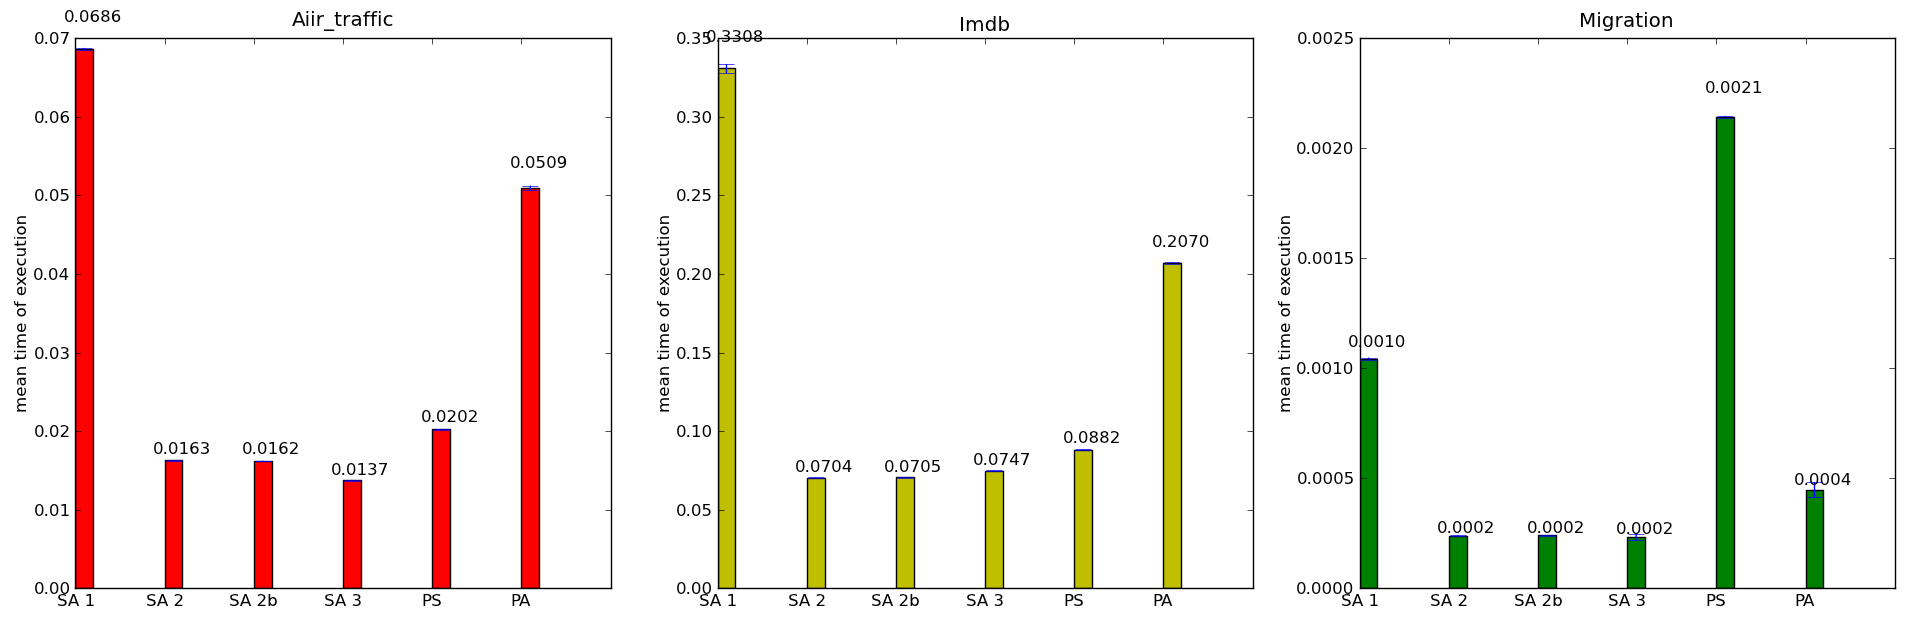
\includegraphics[scale=0.39]{img/histogramme.png}
  \caption{All the mean times of execution}
  \label{histo}
\end{figure}

\underline{\bf Definition of each tag above a bar}
\begin{dinglist}{70}
\item [SA 1]: Tutte sequential asynchronous version on the first data structure;
\item [SA 2]: Tutte sequential asynchronous version on the second data structure;
\item [SA 2b]: Tutte sequential asynchronous version on the second data structure with usage of Vec2f;
\item [SA 3]: Tutte sequential asynchronous version on the third data structure;
\item [PS]: Tutte parallel synchronous version on the second data structure;
\item [PA]: Tutte parallel asynchronous version on the first data structure;
\end{dinglist}

The mean times of computation showed on the figure \ref{histo} have been
obtained with over 1000 executions of each algorithm. The configuration of the
computer having done the executions is :
\begin{description}
\item {Processor}: Intel Core i5-2410M
\item {RAM}: DDRIII 6 GB
\end{description}

One can notice that the best implementation is the sequential asynchronous
version on the second data structure. Also, the parallel implementations
are not the faster, certainly because the number of data to treat is not
great enough.

\subsection{Not planar graph}
The results we get here are not as good as we expected. Although the
computation time is quite improved, the produced graphs are not planar. The
reason is that the provided graph has some fixed nodes inside the
grid. Consequently, after the call of our implementation of the Tutte
Algorithm, some edges crossing (due to those fixed nodes) appear and remove
the planar property of the graph.
\begin{figure}
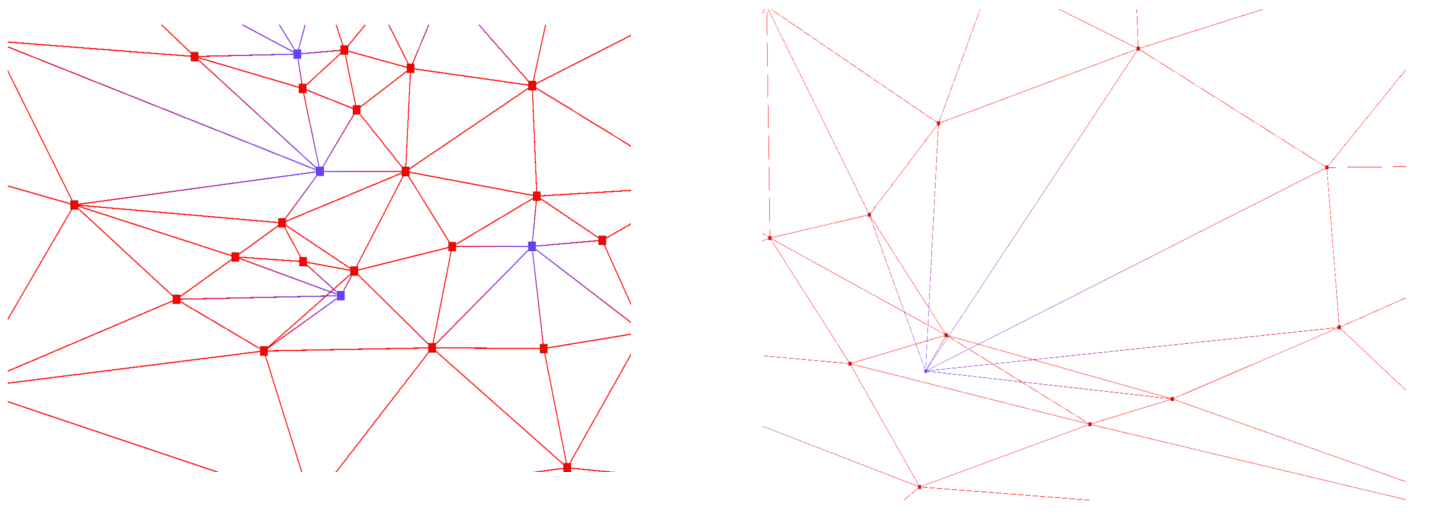
\includegraphics[width=\textwidth]{img/bad_case.png}
\caption{Overview of edge crossing on Aiir Traffic graph}
\end{figure}
As an explanation, we can say that moving nodes tend to be oriented to the 
side which has the highest level of fixed nodes.(see the figure \ref{mauvais_1}). 
With such a graph, a mobile node which is opposite to the side with numerous
edges will move to this side and create an edge-crossing (see the figure \ref{mauvais_2}).

\begin{figure}[!h]
  \begin{minipage}[!h]{.5\linewidth}
   \centering
   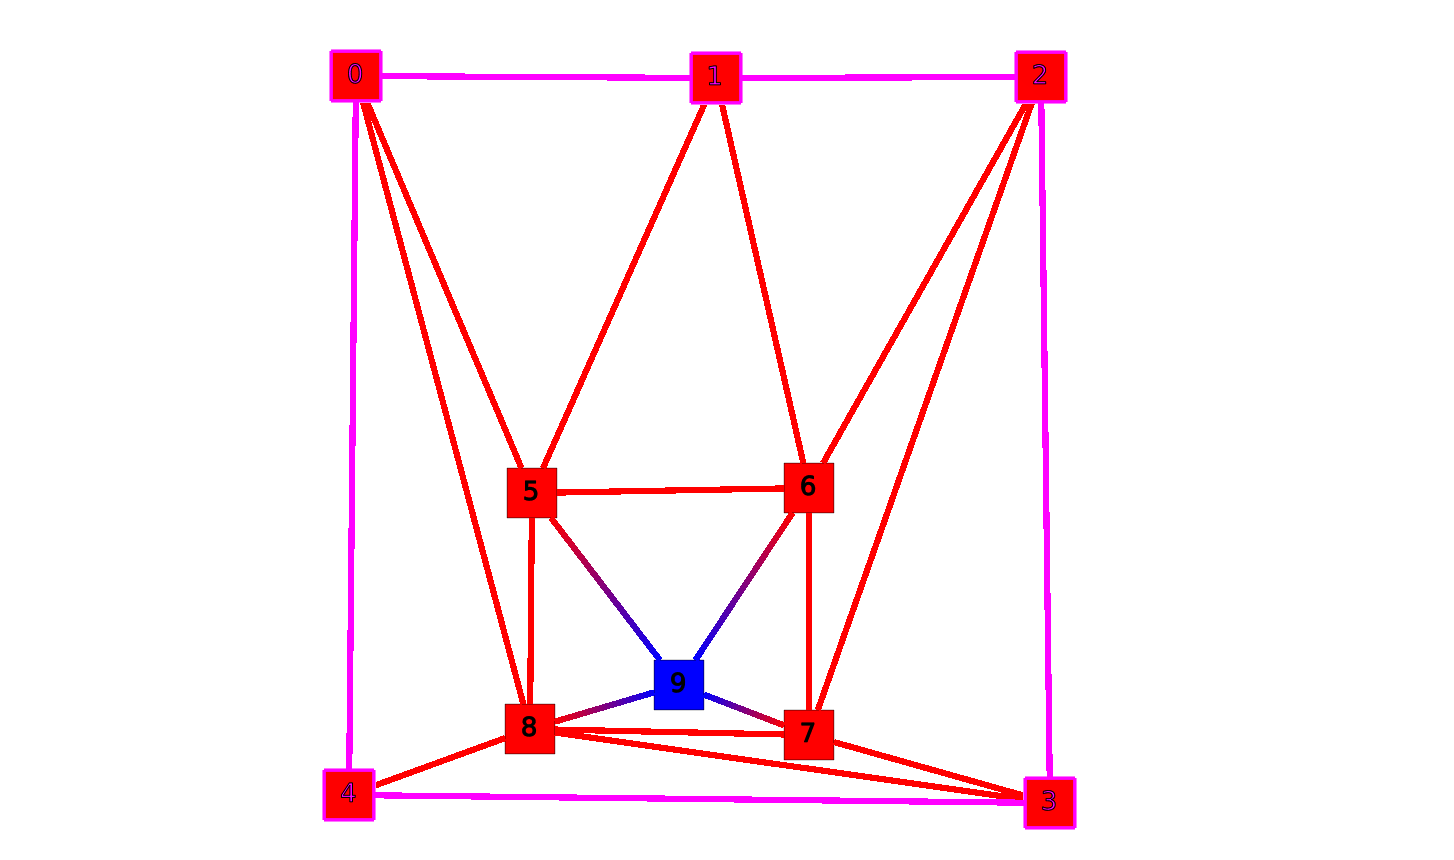
\includegraphics[scale=0.27]{snapshots/constate_fix_init.png}
   \caption{The initial graph. The blue node is fixed}
   \label{mauvais_1}
 \end{minipage} \hfill
 \begin{minipage}[!h]{.45\linewidth}
   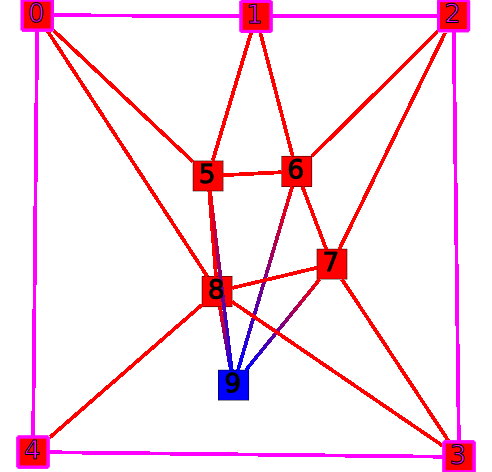
\includegraphics[scale=0.45]{snapshots/constate_probleme.png}
   \caption{The set not correctly modified}
   \label{mauvais_2}
 \end{minipage}
\end{figure}

%\newpage 

You can notice that if all the nodes in the interior of boundaries are mobile, then the graph produced stay planar (see figure \ref{correct_1} and \ref{correct_2}).

\begin{figure}[!h]
  \begin{minipage}[!h]{.5\linewidth}
    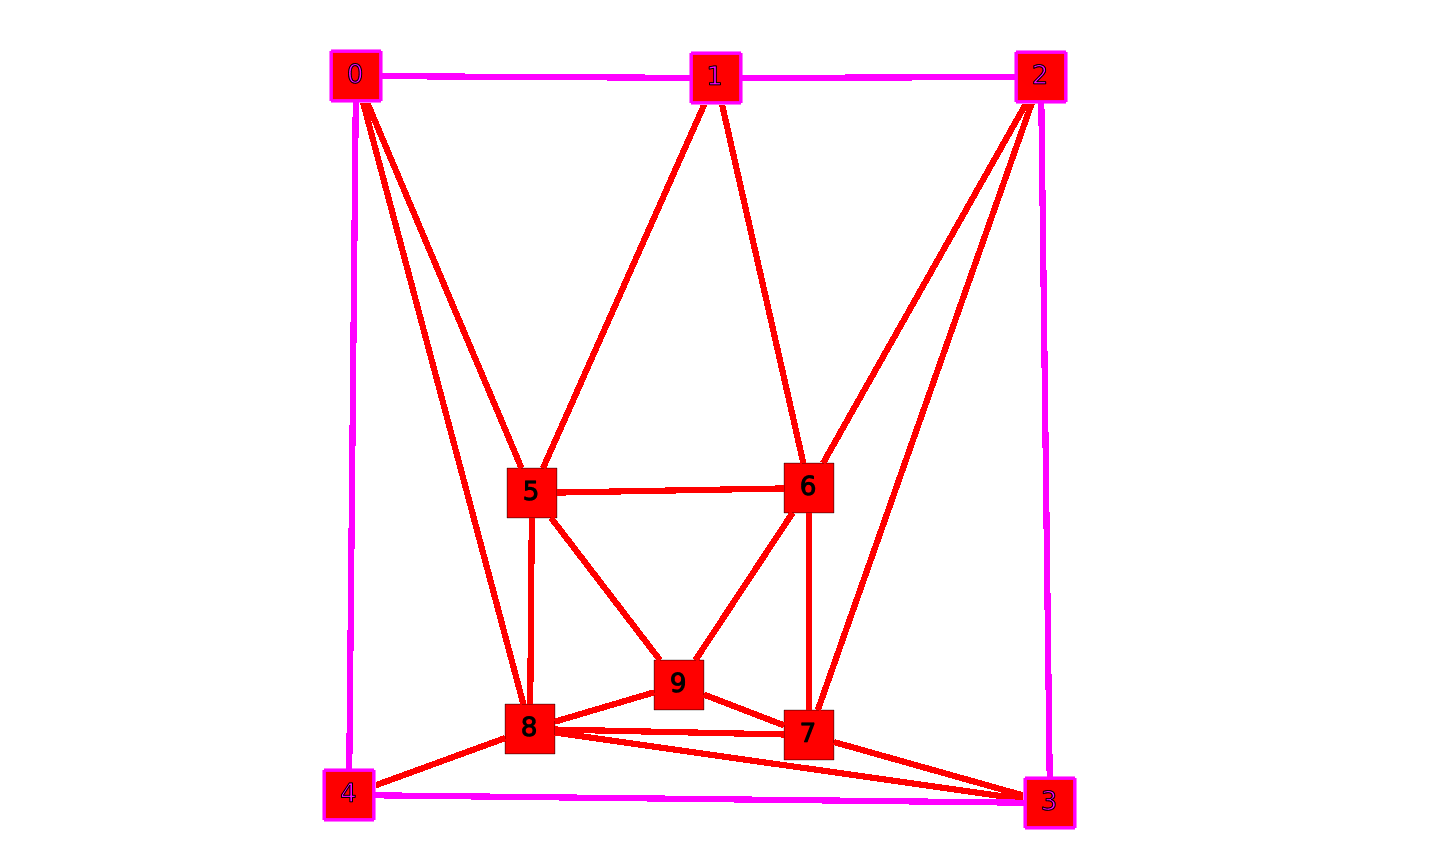
\includegraphics[scale=0.27]{snapshots/constate_mobil_init.png}
    \caption{The initial graph with all interior nodes mobile}
    \label{correct_1}
  \end{minipage}
  \begin{minipage}[!h]{.55\linewidth}
    \centering
    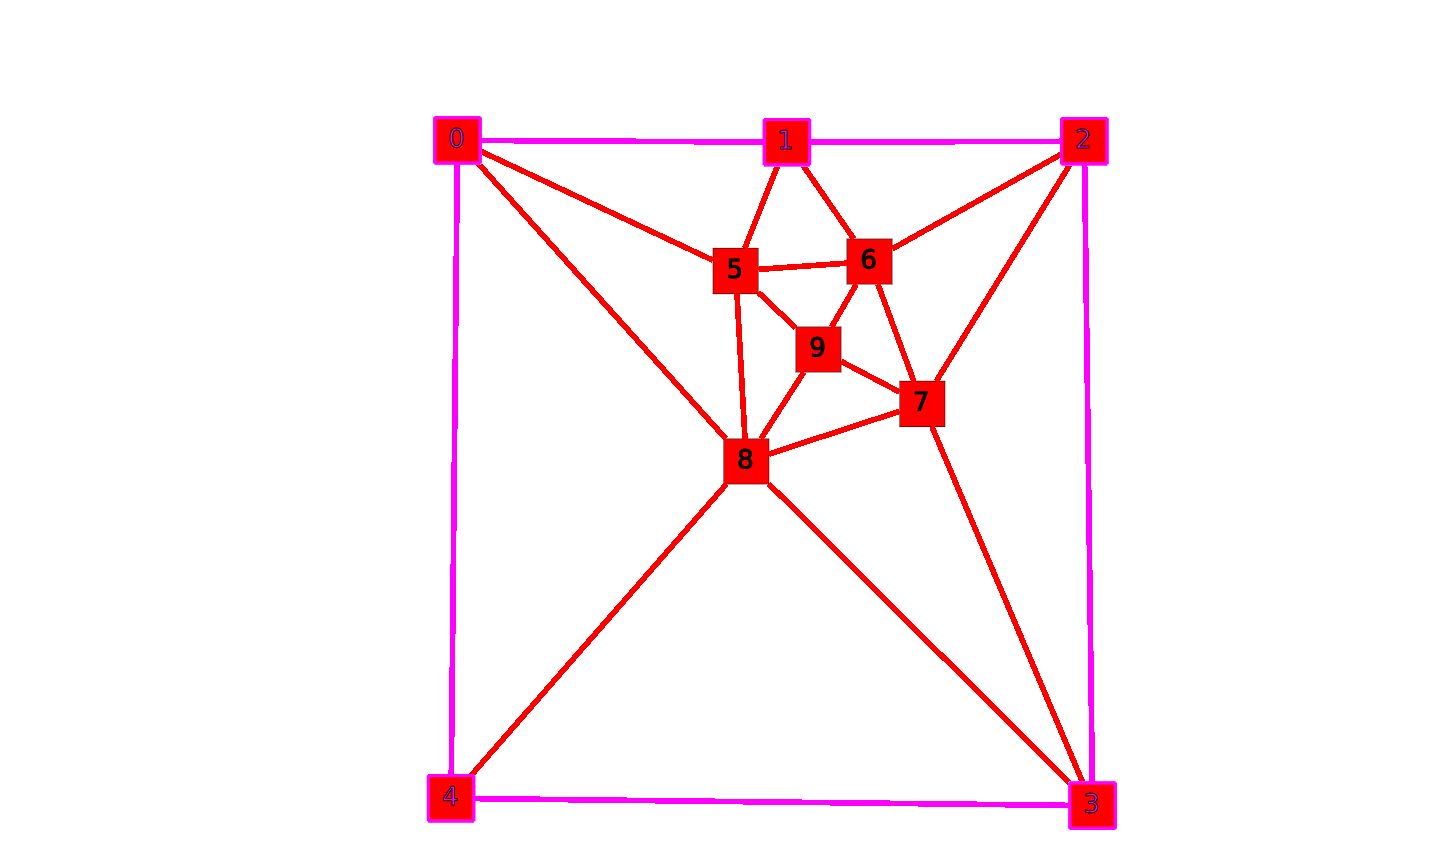
\includegraphics[scale=0.29]{snapshots/constate_nikel.png}
    \caption{The graph correctly modified}
    \label{correct_2}
  \end{minipage} \hfill
\end{figure}


\addcontentsline{toc}{chapter}{Conclusion}
 

%I suggest here to talk about what can be do in the future (there is a quite start of this in my context written in Wiki) 
\begin{thebibliography}{}

\bibitem{pd} A. Lambert, R. Bourqui, and D. Auber. Winding roads: Routing edges
into bundles. \emph{In 12th Eurographics/IEEE-VGTC Symposium on
Visualization (Computer Graphics Forum; Proceedings of EuroVis
2009).} To appear., 2010.

\bibitem{pe} A. Lambert, R. Bourqui, and D. Auber. 3D edge bundling for
geographical data visualization. \emph{In IV ’10: Proceedings of the 14
International Conference on Information Visualisation (IV’09)},
Washington, DC, USA, 2010. IEEE Computer Society.

\bibitem{pb} B. Bollob's. Modern graph theory, \emph{volume 184 of Graduate Texts in Mathematics}. Springer-Verlag, 1998.

\bibitem{pa} E. Colin de Verdière, M. Pocchiola, and G. Vegter. Tutte's Barycenter Method applied to Isotopies. \emph{Computational Geometry: Theory and Applications, 26}, 81–97, 2003.

\bibitem{pf} Gormen, T.H. and Leiserson, C.E. and Rivest, R.L. and Stein, C. Introduction to algorithms. \emph{In MIT press Cambridge, MA}, 16:"Greedy Algorithms", 1990.

\bibitem{pc} William T. Tutte. How to draw a graph. \emph{Proceedings of the London Mathematical Society}, 13:743–768, 1963.

% \bibitem{1} 

% \bibitem{2} 

% \bibitem{3} 

% \bibitem{4} 

% \bibitem{5} 
   
\end{thebibliography}


%%%%%% Liste des annexes %%%%%%%%%%
%% \part{Annexes}
%% \appendix
%% \chapter{Les propriétés \textsf{ACID}}\label{acid}
Les propriétés \textsf{ACID} permettent à un \textsf{SGBD} d'effectuer
des transactions. Par transaction, il faut comprendre une suite
d'opérations qui font passer la \textsf{BDD} d'un état antérieur à un
état postérieur. Les états intermédiaires entre les états avant la
transaction et après la transaction ne sont pas visibles. Ses
propriétés sont les suivantes:

\paragraph{Atomicité:} la suite d'opérations constituant une transaction 
est indivisible. La transaction est entièrement effectuée ou pas du tout. 
Il y a annulation de toute la transaction lorsqu'une des opérations échoue.
S'il est question de modifier une série de valeurs et qu'une modification
échoue alors toutes les valeurs déjà modifiées reprennent leurs anciennes
valeurs. 

\paragraph{Cohérence:} quelque soit l'opération effectuée, la base doit garder
un état cohérent. Toute transaction qui viole par exemple une règle d'intégrité 
échoue. Après la fusion de deux tables, les entrées doivent toutes 
avoir des identités différentes. Si ce n'est pas le cas alors la fusion n'est 
pas effectuée.

\paragraph{Isolation:} chaque transaction est isolée de sorte à ce qu'elle est 
seule peut voir les modifications pendant son exécution. Toute
transaction enclenchée en parallèle d'une autre voit la version des
données antérieure à celle-ci.  Il existe 4 niveaux d'isolation
définis dans le standard \textsf{ANSI/ISO SQL}:
\begin{enumerate}
\item \textsf{Uncommited read ou lectures des données non validées}.
  Ce niveau est le niveau d'isolation le plus léger. Avec un tel
  niveau d'isolation le système se comporte comme s'il n'y en avait
  pas. Les modifications apportées par une transaction non validée
  sont visibles.

\item \textsf{Commited read ou lecture des seules données
  validées}. Les modifications lors d'une transaction ne sont visibles
  que lorsqu'elle termine.  Cependant lors d'une transaction une
  donnée peut changer sans que la transaction en cours en soit
  responsable. Ceci peut arriver, par exemple, lorsqu'une transaction
  en parallèle termine et que ses modifications sont validées.

\item \textsf{Repeatable read ou lecture répétée}. Ce niveau
  fonctionne comme le niveau précédent à la seule différence que
  durant son exécution, une transaction ne voit pas les mises à jour
  effectuées par d'éventuelles transactions qui se sont exécutées en
  parallèle. D'où « \textsf{repeatable read} » pour souligner que pendant une
  transaction, une donnée aura toujours la même valeur en
  lecture si elle n'est pas modifiée par la transaction elle-même.
  Cependant tout nouveau rajout validé de données au système par une
  transaction qui a terminé est visible par toute autre transaction en
  cours.

\item \textsf{Serializable ou sérialisable}. Ce niveau est le niveau
  d'isolation le plus poussé. Le système se comporte comme s'il n'y
  avait qu'une transaction à la fois. Pendant son exécution une
  transaction ne voit ni les mises à jour, ni les rajouts de données
  au système des autres transactions. D'où « \textsf{serializable} » pour
  mettre en relief le caractère d'exécution en série des transactions
  plutôt qu'en parallèle.
\end{enumerate}

\paragraph{Durabilité:} dès lors qu'une transaction est validée, aucune défaillance
du système ne pourra conduire à l'annulation de celle-ci. Les modifications liées à
une transaction validée perdurent et ne sont jamais remises en cause.

\end{document}
